\chapter{Design af brugergrænsefladen}
\label{Design_G}
Dette kapitel beskriver det generelle design af brugergrænsefladen samt de beslutninger, som ligger bag.

\section{Generelle mål}
\label{Design_G_Goals}
Vi har valgt at designe vores brugergrænseflade ud fra reglerne om design af virtuelle vinduer\cite[s. 169]{SL_UID} samt Ease Of Use principperne\cite[s. 9]{SL_UID}. I forbindelse med dette valg har vi sat følgende mål for design:
\begin{itemize}
\item Strømlinet brugergrænseflade
\item Få forskellige skærmbilleder
\item Overblik
\item Effektivt
\end{itemize}

\subsection{Strømlinet brugergrænseflade}
Vi har valgt at designe skærmbillederne med samme grundstruktur. Denne lighed bør gøre det intuitivt at gå fra et skærmbillede til et andet i forbindelse med udførsel af opgaver. Desuden følger det designregel 1\footnote{Few window templates} om få vindueskabeloner.

\subsection{Kort vej fra et opgave til en anden}
Brugergrænsefladen skal gøre det hurtigt og nemt for brugeren at komme fra en opgave til en anden. Dette skal gøres ved at have få skærmbilleder involvereret i en enkelt task (designregel 2\footnote{Few window instances per task.}).

\subsection{Overblik}
Brugeren skal have mulighed for nemt at danne sig overblik over bookinger, udstyr og forplejning (regel 6\footnote{Necessary overview of data}). Derfor skal vi have seperate skærmbilleder, som giver overblik over hver type.

\subsection{Effektivt}
Det skal være effektivt at udføre opgaver for brugere, som anvender systemet ofte.

\section{Grundstruktur}
\label{Design_G_Structure}
Vores brugergrænseflade er delvist inspireret af booking systemer til biografer. Inspirationen består i, at vi laver en visning af lokalerne og får brugeren til grafisk at vælge lokale og tider for deres bookning. Målet var at gøre dette med farvekodning, således at brugeren nemt kunne skelne mellem ledige og optagede lokaler.

\begin{figure}[h!]
  \centering
    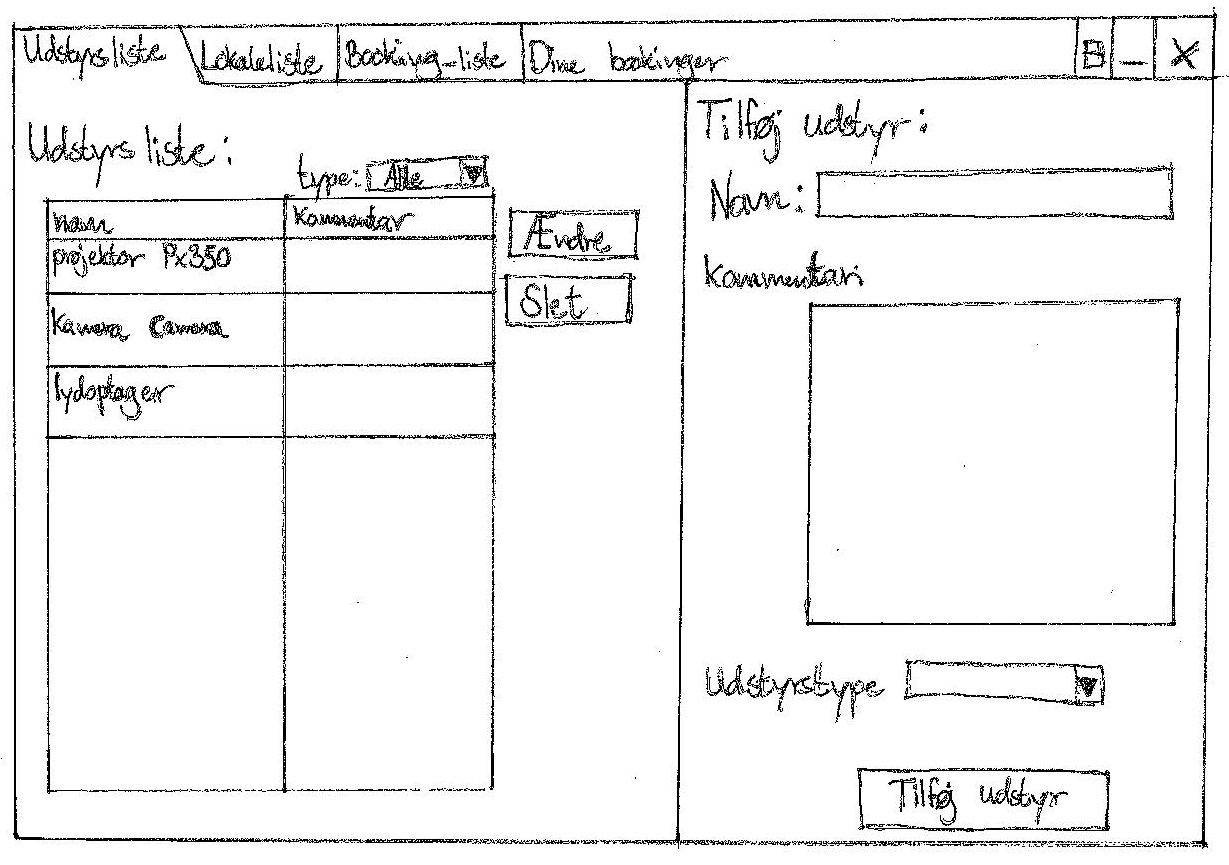
\includegraphics[width=0.5\textwidth]{Appendix/GUI-Prototype/PaperMockup/UdstyrsListe}
  \caption{Screenshot af kino.dk's billet booking brugergrænseflade}
\label{Design_G_Structure_kino}
\end{figure}

Vores første mockup havde et gitter, hvor hver række var et lokale og tiderne var kolonner. Brugerne skulle så klikke i et felt for at vise, at man ønskede at booke på et bestemt tidspunkt. Når man havde valgt de tider og lokaler, man gerne ville booke, skulle man så trykke på en "Book" knap. 
\\Resultatet af vores første usability test viste dog, at denne løsning ikke var intuitiv nok for brugeren. Vi valgte derfor at lave checkboxes inde i hvert felt, således at brugeren skal sætte et hak i de checkboxes, som brugeren vil booke tider ud fra. 
%Namedrop Søren?

Vi anvendte gitterløsningen som grundstrukturen for de fleste skærmbilleder for at følge vores mål om at lave en strømlinet brugergrænseflade. 
\\Til resten af skærmbillederne har vi holdt os til simple strukturer, som kun præsenterer den nødvendige data til at udføre arbejdsopgaven.

\section{Brugergrænsefladens udvikling og udseende}
\label{Design_G_Development}
Vores skærmbilleder er opdelt i tre typer: Gitter, Almindelig og Pop-ups. 
\\Gitterskærmbillederne bruger vi til booking af lokale, forplejning og udstyr samt administration af udstyr og lokaleinventar.
\\Almindelige vinduer anvender vi, hvis man skal ændre noget på et stykke udstyr/inventar eller et lokale.
\\Pop-up skærmbilleder er generelt set advarsler eller fejlbeskeder.

\subsection{Gitterskærmbilledet}
\label{Design_G_Development_Grid}
Figur \ref{Design_G_Development_FinalGrid}, side \pageref{Design_G_Development_FinalGrid} er et screenshot af vores endelige design af booking skærmbilledet.

\begin{figure}[h!]
  \centering
    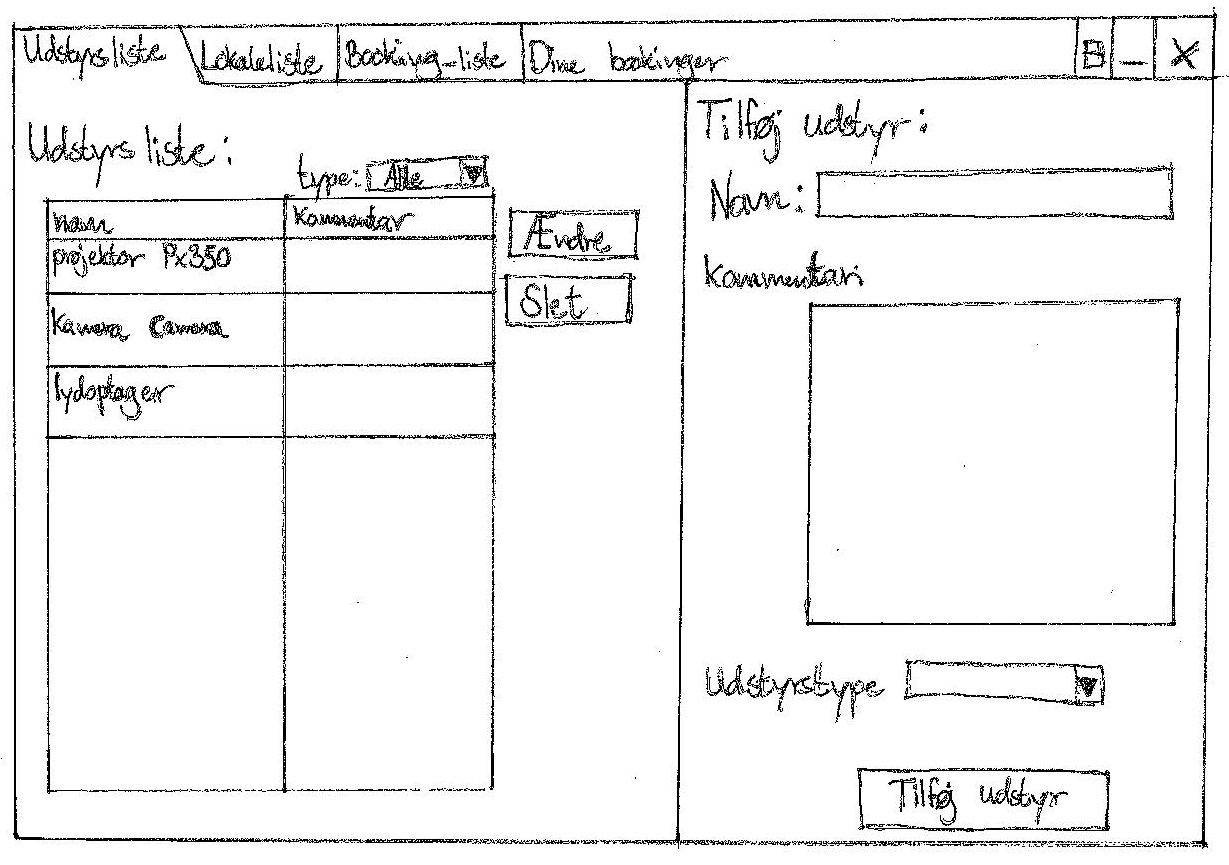
\includegraphics[width=0.5\textwidth]{Appendix/GUI-Prototype/PaperMockup/UdstyrsListe}
  \caption{Den endelige udgave af gitter skærmbilleder til booking}
\label{Design_G_Development_FinalGrid}
\end{figure}

\begin{figure}[h!]
  \centering
    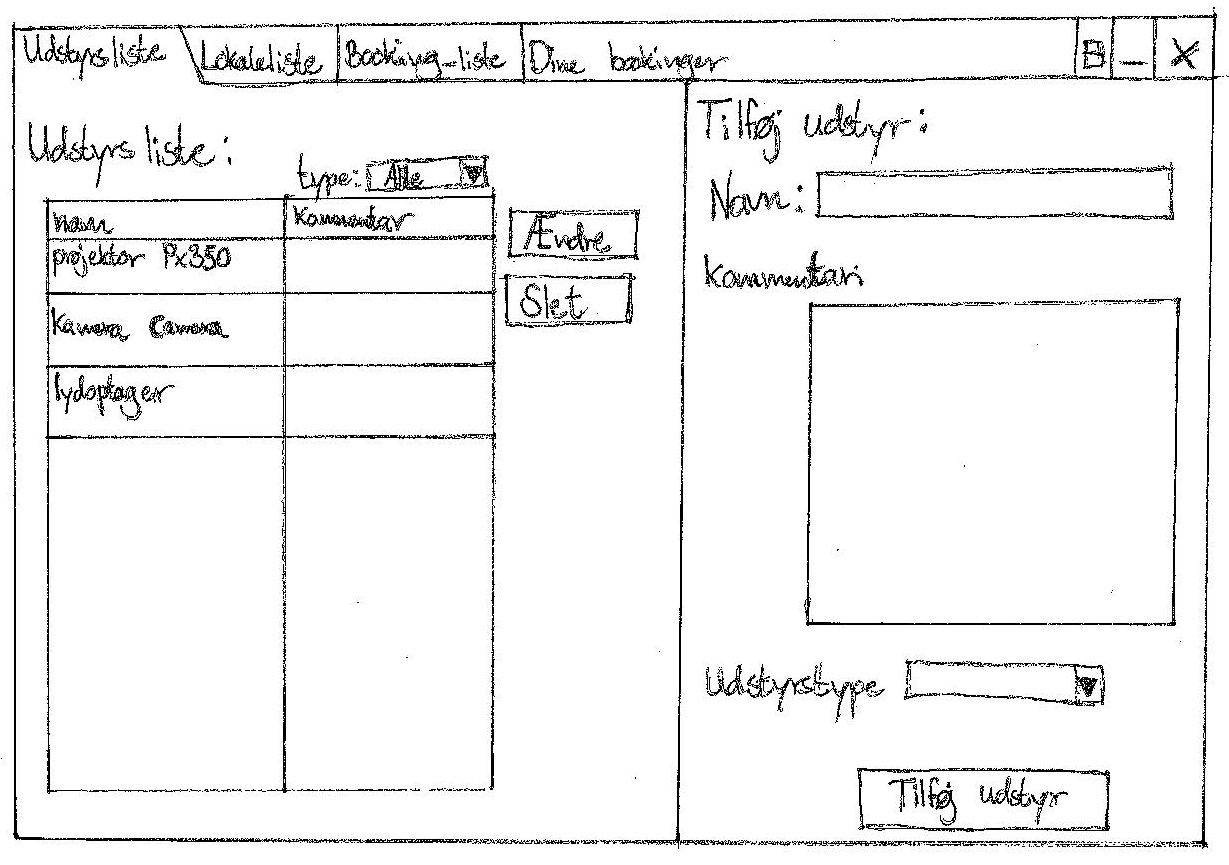
\includegraphics[width=0.5\textwidth]{Appendix/GUI-Prototype/PaperMockup/UdstyrsListe}
  \caption{Første udgave af gitter layoutet}
\label{Design_G_Development_FirstGrid}
\end{figure}

Vi tilføjede efter usability test 1, at udstyr m.m., man har booket, ligger øverst i gitterne, når man får oversigten over fx udstyr. Dette gør det nemt at finde det element, man har booket/bestilt.

Figur \ref{Design_G_Development_FirstGrid}, side \pageref{Design_G_Development_FirstGrid} er det papermockup, som blev brugt til første runde af usability tests. Forskellen på de to skærmbilleder er de checkboxe, som er blevet tilføjet inde i gitteret. 

\subsection{Almindelige skærmbilleder}
\label{Design_G_Development_NormalWindows}
Disse typer af skærmbilleder er primært til administration af udstyr/inventar/lokale og lignende. Et eksempel er skærmbilledet til ændring af et stykke udstyr \ref{Design_G_Development_EquipmentChangeV1}, side \pageref{Design_G_Development_EquipmentChangeV1}. 

I den første udgave i papir mockupen var disse meget simple og manglede noget information om hvad der blev vist. ???????????????? % WTF????
\begin{figure}[h!]
  \centering
    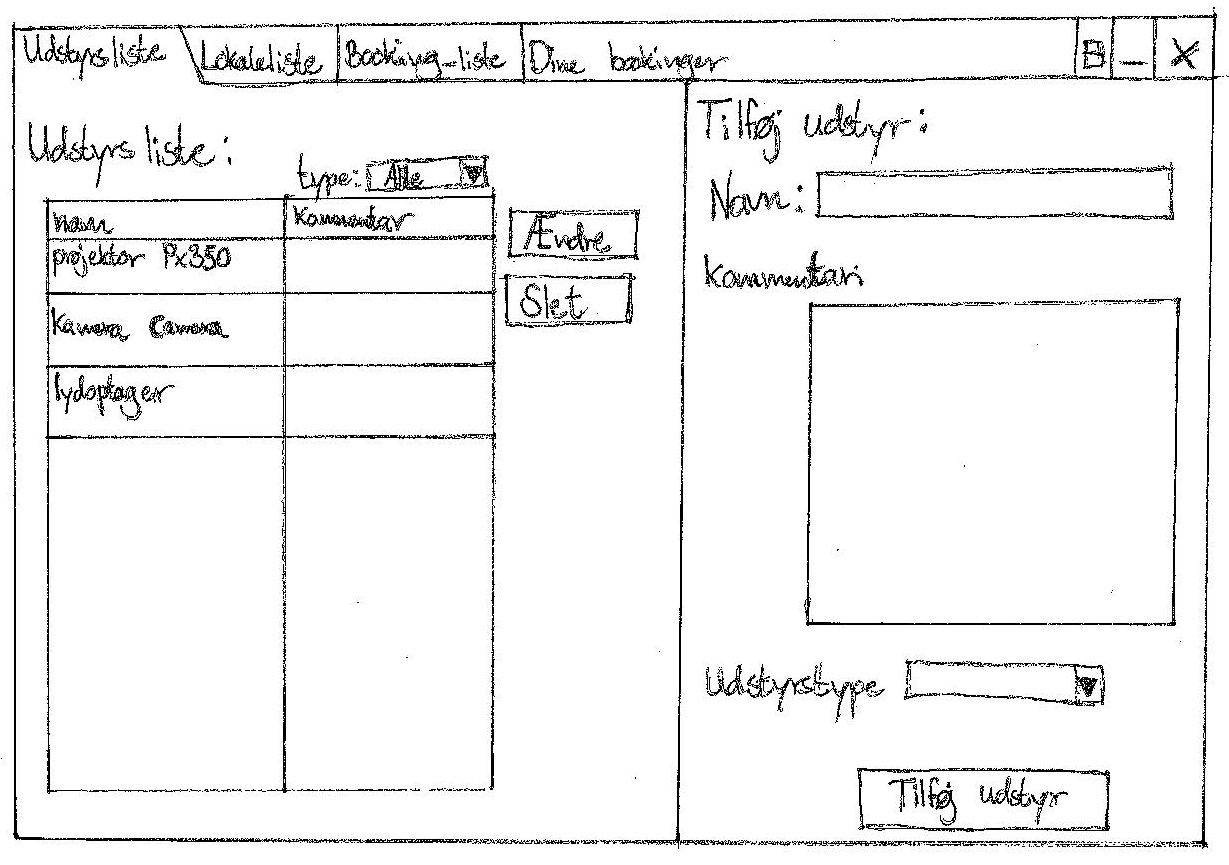
\includegraphics[width=0.5\textwidth]{Appendix/GUI-Prototype/PaperMockup/UdstyrsListe}
  \caption{Første udgave af skærmbilledet til ændring af udstyr}
\label{Design_G_Development_EquipmentChangeV1}
\end{figure} 

Derudover har vi i udviklingen af vores design gået efter at overholede Gestalt-lovene\cite[s. 68]{SL_UID}, specifikt Law of Proximity\footnote{"Pieces that are close together are perceived as belonging together".}. Knapper, som hører til vores gitter, skal ses som hørende til gitteret, og vores "tabs" skal ses som hørende sammen.

%NEED EXAMPLE FOR FUCKS SAKE -^
%BESKRIV TABS